\subsubsection{The challenges performing intra-process communication}


\subsubsection{Message queue}

\paragraph{The premises for designing it}

\paragraph{Various design solutions - Which one chosen and why}

\paragraph{Its design and implementation}

\subsubsection{Impact on design/implementation between before and after the Message Queue}

\subsubsection{Event Driven Programming}

\paragraph{Basic idea}
Event drevet programmering er opgjort af event producenter og event subscribers.
Tråde reagerer på indkommende events, og sover når der ikke sker noget.

Event drevet programmeret er specielt egnet til GUI applikationer hvor user inputs ofte bruges.

Der er flere måder at implementere EDP på. I vores ISU øvelse har vi brugt en MessageQueue hvis funktionalitet er beskrevet ovenfor.
Hvis vi ser på figur~\ref{fig:handlPat} vil vores MessageQueue være være mellemledet før dispatcheren. Dette er smart da det ikke er sikkert at \textit{dispatcher} kan nå at videresende alle events til deres respektive handlers. MessageQueue'en funger derfor som en buffer. 

\begin{figure}[h]
	\centering
	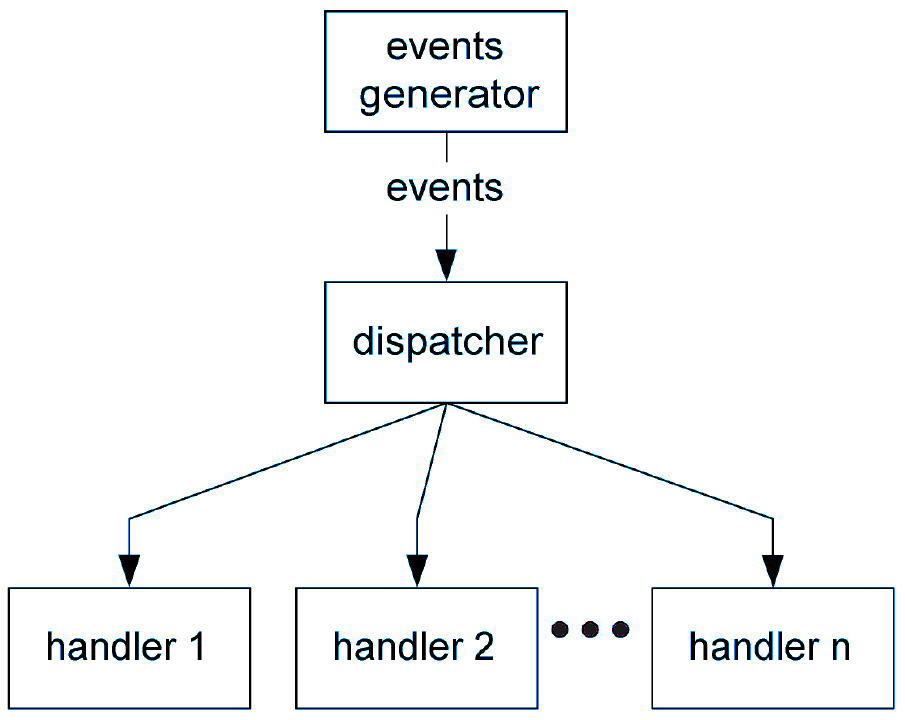
\includegraphics[width=0.6\linewidth]{figs/spm3/handlersPattern}
	\caption{Illustration af et handler pattern}
	\label{fig:handlPat}
\end{figure}

\paragraph{Reactiveness}

\paragraph{Design - e.g. from sequence diagrams to code (or vice versa)}
